\documentclass[aps,reprint,superscriptaddress,nofootinbib]{revtex4-2}

\usepackage[utf8]{inputenc}
\usepackage[english]{babel}
\usepackage{amsmath}
\usepackage{mathtools}
\usepackage{amsfonts}
\usepackage{csquotes}
\usepackage{bm}
\usepackage{indentfirst}
\usepackage{graphicx}
\usepackage{geometry}
\usepackage{minted}
\usepackage{hyperref}
\usepackage{subcaption}
% \usepackage{caption}
\usepackage{algorithm}
\usepackage{algpseudocode}      % For algorithms

\usepackage[format=plain,labelfont=sc, justification=justified,singlelinecheck=false]{caption}
% \captionsetup{justification=raggedright,singlelinecheck=false}

\usepackage{lipsum}
\usepackage{physics}
\usepackage{enumitem}

\graphicspath{ {./figures/} }
\geometry{a4paper,
    left=2cm,
    top=2.5cm,
    bottom=2.5cm,
    right=2cm
}

\newcommand{\Var}{\mathrm{Var}}     % by default \var returns Kronecker delta
\newcommand{\Cov}{\mathrm{Cov}}

\usepackage[T1]{fontenc}
\usepackage{mathptmx}

\begin{document}

\title{A Variational Monte Carlo analysis of Bose-Einstein Condensation of trapped bosons}

\author{Inácio, João}
\affiliation{Department of Physics, University of Oslo, Norway, Sem Sælands vei 24, 0371 Oslo}
\author{Aarstein, Daniel}
\affiliation{Department of Physics, University of Oslo, Norway, Sem Sælands vei 24, 0371 Oslo}

\date{\today}

\begin{abstract}
    In this work, a Variational Monte Carlo code is developed, along with the computational study of Bose-Einstein Condensation on a system of interacting bosons, confined to a harmonic trap. We compare the sampling efficiency of standard Metropolis sampling and Metropolis sampling with importance sampling by the Fokker-Planck and Langevin equations. We compute one-body densities for the non-interacting and interacting systems. All of the code and results used in this report can be found at this \url{https://github.com/jgci2000/FYS4411-vmc} GitHub repository.
\end{abstract}

\maketitle

    In this project, we try to reproduce the results in \cite{bec-trapped-bosons}. That is, perform a computational study of a hard-sphere trapped Bose gas, through Variational Monte Carlo. This Bose gas, consists of hard-sphere bosons (with radius \(a\)), interacting via a hard-core potential. 
    
    Monte Carlo methods, take advantage of the equilibrium state of a stochastic model, called Markov chain, in order to simulate a real life experiment. That is, we will generate a chain of events and take measurements of the desired quantities at each link in the chain. Through this, we can obtain an estimation of the energy of our system, for example. To generate this chain, we start with a random state and make small changes to it, accepting this changes with a weighted probability. Variational Monte Carlo, uses this sampling process, to sample the energy for a given trial wavefunction. This trial wavefunction depends on some parameters (called variational parameters), for which we can optimize for the lowest energy state. We then improve this sampling method by introducing a new way of sampling the phase space. This will allow for a faster convergence. Lastly, we compute one-body densities for the particles in the interacting system.

\section*{Variational Monte Carlo}

    \textit{Variational Monte Carlo} (VMC) is a quantum Monte Carlo method that applies the variational principle in order to estimate the ground state of a quantum system. With the variational method we can try to guess the ground state wavefunction, \(E_0\), for a given quantum system, with a Hamiltonian \(H\) \cite{sakurai}. Then given a trial wavefunction \(\ket{\Psi_T}\), the variational method gives us
    \begin{equation} \label{eq:var_method}
        E_0 \leq E = \frac{\bra{\Psi_T} H \ket{\Psi_T}}{\bra{\Psi_T} \ket{\Psi_T}} = \frac{\int d\bm R \Psi_{T}^{*} H \Psi_T}{\int d\bm R \Psi_{T}^{*} \Psi_T}.
    \end{equation}
    In the case that the trial wavefunction is the ground state wavefunction, we will have \(E_0 = E\). The most difficult part of this method is finding a correct trial function that minimizes the energy. During this process it is crucial that we use our physical intuition about the system. For a few select systems, this is possible to compute analytically. One can check if a trial wavefunction is close to the ground state wavefunction by computing the variance of the estimated energy,
    \begin{equation*}
        \sigma^2_E =  \frac{\bra{\Psi_T} H^2 \ket{\Psi_T}}{\bra{\Psi_T} \ket{\Psi_T}}  - \left( \frac{\bra{\Psi_T} H \ket{\Psi_T}}{\bra{\Psi_T} \ket{\Psi_T}} \right)^2
    \end{equation*}
    For the exact ground state this should be zero. Thus our task is to find the wavefunction that minimizes the variance of the energy.
    
    In our case, we have a fixed wavefunction and want to vary some parameters (called variational parameters), so that the trial wavefunction best fits the ground state one. This is another approach as trying different wavefunctions. So, let us define a trial wavefunction as \(\Psi_T(\bm R; \bm \alpha)\), where \(\bm R = \{\bm r_1, \bm r_2, \ldots, \bm r_N \}\) is the position vector of all particles in the system and \(\bm \alpha = \{\alpha, \beta, \ldots \}\) are the variational parameters of the wavefunction. We can thus write the variational method as
    \begin{equation} \label{eq:vmc_use}
        E_0 \leq E(\bm \alpha) = \frac{\int d\bm R \Psi_T^*(\bm R; \bm \alpha) H \Psi_T(\bm R; \bm \alpha)}{\int d\bm R \left| \Psi_T(\bm R; \bm \alpha) \right|^2}.
    \end{equation}
    Another type of approach is to use a neural network as the trial wavefunction. This way, instead of designing an expression for the trial wavefunction (which might not even be possible in some cases), we can just use a blank neural network and train it so it fits better the problem at hand \cite{nn_vmc_nuclei, many_body_ml}.
    
    To solve this problem, one innocent approach might be to use Gaussian integration techniques in order to solve the integrals in Equation \eqref{eq:var_method}. This turns out to be quite heavy computationally, since if we have \(N\) particles with \(d\) degrees of freedom, we would be solving \(dN\) dimensional integrals, and this requires an evaluation of the integrand a total of \(m^{dN}\) times \cite{curse_dim}, where \(m\) is the number of quadrature points in one of the dimensions. This number becomes very large when we want a fine integration domain and a high number of particles. So, to evaluate these multi-dimensional integrals we use the \textit{Monte Carlo} method \cite{landau_binder_2014} as this method does not suffer form the so-called curse of dimensionality.
    
\subsection*{Monte Carlo Integration}

    The Monte Carlo (MC) method is able to evaluate integrals by extracting \(M\) samples from the integrand at random points in the integration space,
    \begin{equation*}
        y = \int_{\mathbb{R}} dx f(x) \approx \frac{1}{M} \sum_{i=1}^{M} f(x_i).
    \end{equation*}
    This method is exact in the limit \(M \rightarrow \infty\). If, however, we let \(f(x) = O(x) p(x)\), where \(p(x)\) is a probability distribution, we can compute the expectation value of some variable \(O\), \(\langle O \rangle\) by
    \begin{equation*}
        \langle O \rangle = \int_{\mathbb{R}} dx O(x)p(x) \approx \frac{1}{M} \sum_{i=1}^{M} O(x_i).
    \end{equation*}
    
    To take advantage of the MC method, we need to define a probability density function. Since \(\left| \Psi_T(\bm R; \bm \alpha) \right|^2\) already defines a probability density, we are able to use that. More specifically, we are interested in a normalized probability density, so
    \begin{equation} \label{eq:pdf_vmc}
        P(\bm R; \bm \alpha) = \frac{\left| \Psi_T(\bm R; \bm \alpha) \right|^2}{\int d\bm R \left| \Psi_T(\bm R; \bm \alpha) \right|^2}
    \end{equation}
    is our probability density. This means that our estimator for the energy is  
    \begin{equation*}
        E_L(\alpha) = \frac{1}{\Psi_T(\bm R; \bm \alpha)} H \Psi_T(\bm R; \bm \alpha)
    \end{equation*}
    the local energy. In general, we can define the estimator of any observable \(O\) as \(O_L(\alpha) = \frac{1}{\Psi_T(\bm R; \bm \alpha)} O \Psi_T(\bm R; \bm \alpha)\), where \(O_L\) is the local version of the observable. We can finally rewrite once more the variational principle as 
    \begin{equation*}
        E(\bm \alpha) \approx \frac{1}{M} \sum_{i=1}^{M} E_L(\bm R_i, \bm \alpha)
    \end{equation*}
    
\subsection*{Metropolis method}

    Having defined our estimators and probability distribution, we just need an efficient way to sample the position space. For this we use the \textit{Metropolis method} \cite{metropolis_1953}. The Metropolis method is a way to efficiently sample probability distributions using Markov chains. It has seen many applications from the study of magnetism, quantum ensembles, protein-folding and machine learning.
    
    A \textit{Markov chain} is a stochastic model that describes a series of events, in which the probability of transitioning to the next state depends only on the current state. Let us define \(P_i^{(n)}\) as the probability of being in state \(i\) on step \(n\), \(T_{i \rightarrow j}\) as the probability of transitioning from state \(i\) to state \(j\) and \(A_{i \rightarrow j}\) as the probability of accepting the move from state \(i\) to \(j\), we also required that \(A_{i \rightarrow j} = 1 - A_{j \rightarrow i}\). One of the properties of \(T\) is that \(\sum_j T_{i \rightarrow j} = 1\). By the definition of a Markov chain, we know that the probability of being in state \(i\) at time \(n\) is the sum of the probabilities of being in some other state \(j\) at time \(n-1\) and accepting the move, together with the probability of being already on state \(i\) and rejecting the move to a new state \(j\). Mathematically, this can be written as 
    \begin{align*}
        P_i^{(n)} = \sum_j \left[ P_j^{(n-1)} T_{j \rightarrow i} A_{j \rightarrow i} + P_i^{(n-1)} T_{i \rightarrow j} (1 - A_{i \rightarrow j}) \right] \\
        = P_i^{(n-1)} + \sum_j \left[ P_j^{(n-1)} T_{j \rightarrow i} A_{j \rightarrow i} - P_i^{(n-1)} T_{i \rightarrow j} A_{i \rightarrow j} \right]
    \end{align*}
    Letting \(n \rightarrow \infty\) (stationary state), we define the time independent probability \(P_i \leftarrow P_i^{(n)}\) (also called the stationary distribution). The last equation is then
    \begin{equation*}
        \sum_j \left[ P_j T_{j \rightarrow i} A_{j \rightarrow i} - P_i T_{i \rightarrow j} A_{i \rightarrow j} \right] = 0
    \end{equation*}
    and it is known as the master equation, which provides the global balance conditions. If we look at one element of the sum,
    \begin{equation*}
        P_j T_{j \rightarrow i} A_{j \rightarrow i} = P_i T_{i \rightarrow j} A_{i \rightarrow j}
    \end{equation*}
    then we have the detailed balance condition for our Markov chain. The Metropolis choice is to maximize the acceptance probabilities, so 
    \begin{equation*}
        A_{i \rightarrow j} = \min \left\{ 1, \frac{P_j T_{j \rightarrow i}}{P_i T_{i \rightarrow j}} \right\}.
    \end{equation*}
    
    In our case, \(P_i = P(\bm R_i; \bm \alpha)\), and we set \(T_{i \rightarrow j} = 1\). So our Metropolis ratio becomes 
    \begin{equation} \label{eq:acepp_met}
        A_{i \rightarrow i+1} = \min \left( 1, q(\bm R_{i+1}, \bm R_i) \right),
    \end{equation}
    with 
    \begin{equation} \label{eq:q_met}
        q(\bm R_{i+1}, \bm R_i) = \frac{\left| \Psi_T(\bm R_{i+1}; \bm \alpha) \right|^2}{\left| \Psi_T(\bm R_{i}; \bm \alpha) \right|^2}.
    \end{equation}
    This model assumes that the Markov chain is already on the stationary state. This however is not true for the first steps of the simulation, since the positions of the particles are initialized randomly. We then have to let the system reach the equilibrium stage and only after that, we can start to sample the desired observables. We do this by setting a percentage of the total MC cycles for the equilibration process, i.e., not sampling for some steps. This way, the Metropolis method can be condensed into the following steps:
    \begin{enumerate}[noitemsep,nolistsep]
        \item Start with the positions vector \(\bm R\) uniformly distributed. Here we choose values in the interval \([-0.5, 0.5]\);
        \item Update the system by selecting one particle, \(k\), at random and update its position by \(\bm r_k^{(i+1)} = \bm r_k^{(i)} + p \times \text{step}\_\text{length} \), where \(\text{step}\_\text{length}\) is the maximum distance you can move one particle, and \(p\) is a uniformly distributed random variable on the interval \([-1, 1]\);
        \item Accept or reject the move with the acceptance criteria in Equations \eqref{eq:acepp_met} and \eqref{eq:q_met}. This is, compute the ratio \(q\) and generate a random variable \(r\) uniformly distribute in \([0, 1]\). If \(r \leq q\), accept \(r_k \leftarrow r_k^{(i+1)}\), else reject \(r_k \leftarrow r_k^{(i)}\);
        \item If the system has reach equilibrium, measure the desired quantities;
        \item Repeat the last three steps until you have the desired number of samples.
    \end{enumerate}
    
\subsection*{Metropolis with Importance Sampling}

    Inherently, Metropolis sampling does not take into account where are the most likely to find a particle at, since we update particles by a random value. This results in wasted cycles, since if the random update does not favour the system, it will not be accepted by the criteria. Instead we introduce a new way of updating the particle trajectory in the coordinate space. This approach is based on the Fokker-Planck and Langevin equations. We start with the Fokker-Planck equation
    \begin{equation*}
        \frac{\partial P(\bm R, t)}{\partial t} = D \nabla \cdot \left(\nabla - \bm F \right)P(\bm R, t).
    \end{equation*}
    This equations describes the evolution in time of a probability density function. In our case it is Equation \eqref{eq:pdf_vmc}. Here \(D\) is the diffusion constant that we set to \(\frac{1}{2}\), and \(\bm F\) is a drift force. In our case, this drift force is defined by
    \begin{equation*}
        \bm F = \sum_{k=1}^N \bm F_k (\bm R) = \sum_{k=1}^N \frac{2 \nabla_k \Psi_T(\bm R; \bm \alpha)}{\Psi_T(\bm R; \bm \alpha)},
    \end{equation*}
    where \(\nabla_k\) is the gradient with respect to particle \(k\).
    
    We use the Langevin equation to find the new positions in the coordinate space.
    \begin{equation*}
        \frac{\partial \bm R}{\partial t} = D \bm F(\bm R) + \eta
    \end{equation*}
    Here \(\eta\) is a uniformly distributed random variable in the interval \([0, 1]\). We can use Euler's method to solve this equation and we are left with 
    \begin{equation} \label{eq:langevin}
        \bm R_{i+1} = \bm R_i + D \bm F(\bm R_i) \Delta t + \xi \sqrt{\Delta t},
    \end{equation}
    where \(\xi\) is a Gaussian variable with mean \(0\) and standard deviation \(1\). Usually \(\Delta t \in [0.001, 0.01]\).
    
    The new acceptance ratio will take into account the new updating scheme for the particle positions through the evaluation of the Green's function of the Fokker-Planck equation
    \begin{equation} \label{eq:gfs}
        G(\bm x, \bm y) = \frac{1}{(4 \pi D \Delta t)^{dN/2}} \exp \left( \frac{-(\bm y - \bm x - \Delta t \bm F(\bm x))^2}{4 D \Delta t} \right).
    \end{equation}
    This way,
    \begin{equation*}
        q(\bm R_{i+1}, \bm R_i) = \frac{G(\bm R_i, \bm R_{i + 1}) \left| \Psi_T(\bm R_{i+1}; \bm \alpha) \right|^2}{G(\bm R_{i+1}, \bm R_i) \left| \Psi_T(\bm R_{i}; \bm \alpha) \right|^2}.
    \end{equation*}
    With this new sampling procedure, we expect that the acceptance ratio of new configurations will be higher than with Metropolis sampling. One disadvantage of this new scheme is that it requires more computational time to update the particles and compute the acceptance criteria \(q\). 

\subsection*{Optimizing the Energy}

    Our aim is to find the variational parameters that minimize the local energy and run a big MC calculation for those parameters. Since we know that the local energy is a convex function for the variational parameters, Equation \eqref{eq:vmc_use}, then we can employ some optimization algorithm to find the optimal variational parameters and run a longer calculation for the found parameters. This allows us to perform a better search for the best variational parameters. Our goal is thus to find
    \begin{equation*}
        \text{argmin}\ E(\bm \alpha),
    \end{equation*}
    or, the variational parameters where \(\nabla_{\bm \alpha} E(\bm \alpha) = 0\). This is an example of a classical minimization problem, where we can employ \textit{Newton's method} \cite{num_anal_mayers}
    \begin{equation*}
        \bm{\alpha}^{(k+1)}=\bm{\alpha}^{(k)}-\big(H_E(\bm{\alpha}^{(k)})\big)^{-1}\nabla E(\bm{\alpha}^{(k)}),
    \end{equation*}
    where \(\bm{\alpha}^{(k)}\) are the variational parameters at iteration \(k\), and \(H_E(\bm{\alpha}^{(k)})\) is the Hessian matrix of \(E(\bm \alpha)\) evaluated at \(\bm{\alpha}^{(k)}\). Newton's method converges quadratically \cite{num_anal_mayers}, however it is computationally expensive, since we have to compute the Hessian matrix and invert it, every iteration. This term can be replaced by some coefficient \(\eta\), with the restriction that it is lower than the largest eigenvalue of \(H_E(\bm{\alpha})\). This method is called \textit{Gradient Descent}. 
    \begin{equation*}
        \bm{\alpha}^{(k+1)}=\bm{\alpha}^{(k)}-\eta \nabla E(\bm{\alpha}^{(k)})
    \end{equation*}
    
    In order to compute the gradient of the local energy, we can use the finite difference method,
    \begin{equation*}
        \frac{\partial E}{\partial \alpha_i} = \frac{E(\alpha_i + h) - E(\alpha_i - h)}{2h} + \mathcal{O}(h^2).
    \end{equation*}
    With this method we can estimate \(E(\alpha_i \pm h)\) by a small MC computation. One step-back opposed to using an analytical expression is that if \(h\) is small (\(h \sim 10^{-4}\)), the small deviations in the MC estimation might give the derivative a different sign. This poses a problem in the gradient descent method, because instead of iterating in a descent direction we iterate in a ascent direction. To avoid this, we should keep \(h\) relatively large, so that the values of \(\alpha_i \pm h\) are sufficiently apart that this does not become an issue.
    
\section*{Statistical Analysis}

    The statistic of the computed mean energy of the system is not very useful without knowing the accompanying uncertainty. Hence we wish to calculate the variance and the standard deviation of the mean energy. A smaller standard deviation indicates a stronger certainty in the statistic. However, seeing as our data is correlated (due to the nature of our random number generator), the calculation of the variance and standard deviation will be skewed.
    
    In this project the true mean energy is approximated by the mean of our sample of measurements, $m$, where
    
    \begin{equation*}
        m = \frac{1}{N}\sum_{i = 1}^N x_i
    \end{equation*}
    
    The $x_i$'s are values of the relevant Monte Carlo simulation.
    Calculating the variance and standard deviation of the mean energy is the reduced to calculating it for $m$. The variance of the sample mean is given by
    
    \begin{align*}
        \Var(m) &= \langle{m^2}\rangle - \langle{m}\rangle^2
    \end{align*}
    Lets start with calculating $\langle m \rangle^2$. Note that since the sample mean is given by a finite sum, thus
    
    \begin{align*}
        \langle m \rangle &= \big\langle \frac{1}{N}\sum_{i=1}^N x_i \big\rangle \\
        &= \frac{1}{N}\sum_{i=1}^N \langle x_i \rangle
    \end{align*}
    
    This quantity squared is then 
    
    \begin{align*}
        \langle m \rangle ^2 &= \frac{1}{N^2}\qty(\sum_{i=1}^N\langle x_i \rangle)^2 \\
        &= \frac{1}{N^2}\sum_{i=1}^N\sum_{j=1}^N\langle x_i \rangle \langle x_j \rangle
    \end{align*}
    
    Similarly, the expectation value of the sample mean square is then given by
    
    \begin{align*}
        \langle m^2 \rangle &= \langle \frac{1}{N^2}\sum_{i=1}^N\sum_{j=1}^N x_i x_j \rangle \\
        &= \frac{1}{N^2}\sum_{i=1}^N\sum_{j=1}^N\langle x_i x_j \rangle
    \end{align*}
    
    In total we then have
    
    \begin{align*}
        \Var(m) &= \frac{1}{N^2}\sum_{i=1}^N\sum_{j=1}^N\langle x_i x_j \rangle - 
        \frac{1}{N^2}\sum_{i=1}^N\sum_{j=1}^N\langle x_i \rangle \langle x_j \rangle \\
        &= \frac{1}{N^2}\sum_{i=1}^N\sum_{j=1}^N\qty(\langle x_i x_j \rangle - \langle x_i \rangle \langle x_j \rangle) \\
        &= \frac{1}{N^2}\sum_{i=1}^N\sum_{j=1}^N\Cov(x_i, x_j)
    \end{align*}
    
    Where we have noticed that the term in the sum is simply the covariance between $x_i$ and $x_j$. In the case that $i=j$ the covariance is the variance of $x_i$, so that term may be extracted
    
    \begin{equation}\label{eq:var_mean}
        \Var(m) = \frac{1}{N^2}\sum_{i=1}^N\Var(x_i) + \frac{2}{N^2}\sum_{i=1}^{N-1}\sum_{j=i+1}^N\Cov(x_i, x_j)
    \end{equation}
    
    Using that $\Cov(x_i, x_j) = \Cov(x_j, x_i)$ there is no need to count the combination twice, hence the $j$ index only goes from $i+1$ to $N$.\\
    If we now define the function $\gamma(h)$ which calculates the covariance between elements separated by a distance $h = \abs{i - j}$ as
    
    \begin{align*}
        \gamma(h) = \Cov(x_i, x_j) = \Cov(x_i, x_{i+h})
    \end{align*}
    
    Note that for $h = 0$ we have $\gamma(0) = \Cov(x_i, x_i) = \Var(x_i)$. Using this fact as well as replacing the double sum in \ref{eq:var_mean} with an appropriate expression using the $\gamma$ function, we get
    
    \begin{align*}
        \Var(m) &= \frac{1}{N^2}N\gamma(0) + \frac{2}{N^2}\sum_{h=1}^{N-1}\qty(N-h)\gamma(h) \\
        &= \frac{\gamma(0)}{N} + \frac{2}{N}\sum_{h=1}^{N-1}\qty(1-\frac{h}{N})\gamma(h)
    \end{align*}
    
    By introducing the error term $e = \frac{2}{N}\sum_{h=1}^{N-1}\qty(1-\frac{h}{N})\gamma(h)$ we then have that the variance of the sample mean is given by
    
    \begin{equation} \label{eq:var_err}
        \Var(m) = \sigma^2(m) = \frac{\sigma^2}{N} + e
    \end{equation}
    
    From this it is evident that the error term provides some correction because of the correlation, for uncorrelated data points the variance is given by $\sigma^2/N$.
    
    Alternatively, we may continue the calculation by having $\gamma(0)/N$ as a common factor in order to obtain
    \begin{align*}
        \Var(m) &= \frac{\gamma(0)}{N}\qty[1 + 2\sum_{h=1}^{N-1}\qty(1 - \frac{h}{N})\frac{\gamma(h)}{\gamma(0)}]
    \end{align*}
    
    The scaled covariance function is by definition the autocorrelation function, here given by
    
    \begin{equation*}
        \kappa_h = \frac{\gamma(h)}{\gamma(0)} = \frac{\gamma(h)}{\Var(x_i)}
    \end{equation*}
    
    By defining the variable $\tau = \qty[1 + 2\sum_{h=1}^{N-1}\qty(1-\frac{h}{N})\kappa_h]$ (corresponding to autocorrelation time) and inserting into our expression for the variance of the sample mean, we (finally) have
     
    \begin{equation*}
        \Var(m) = \sigma^2(m) = \frac{\sigma^2}{N}\tau
    \end{equation*}
   
    % I made a figure like the one they had that made no sense. See the last one. I think it shows the equilibration process of the Markov Chain.
    %In order to correct for this we implemented the resampling method known as the Blocking method \cite{blocking}.
    
    Using this one may get an exact standard deviation of our sample mean. However, calculating $\tau$ is quite costly as its a covariance over a double sum. Because of this we wish to omit the calculation in its entirety.  This is where blocking enters the picture! 

%\subsection*{Resampling}

    %In general, a resampling method can be used to estimate the precision of a sample statistic (mean, variance, etc.) by using a subset or reordering of the data which is already generated. This is useful if obtaining data is costly, either when it comes to time or computing resources.
    
\subsection*{Blocking}
    
    The Blocking method is used to de-correlate data, by means of applying a so-called blocking transformation. This procedure can be repeated until a sufficiently good approximation of the variance of the mean has been found.
    
    It can be shown \cite{MJ_Blocking} that by performing a sufficient amount of blocking transformations the error term in \ref{eq:var_err} goes to zero. This, however, might require quite the amount of data, due to a single transformation halving the datasize. In general the method works best for arrays with size $2^d$ where $d$ is an integer.
    
    The method utilizes some basic statistics, namely the variance of the blocked data
    
    \begin{equation*}
        \sigma_i^2 = \frac{1}{n_i}\sum_{j = 1}^{n_i}\qty(x_j - \bar{x}_i^2)
    \end{equation*}
    
    and an approximation to the autocovariance. It suffices to use the first order autocovariance, that is set $h = 1$. $\gamma_i(1)$ is then given by
    
    \begin{equation*}
        \gamma_i(1) = \frac{1}{n_i}\sum_{j=1}^{n_i}\qty(x_j - \bar{x}_i)\qty(x_{j+1} - \bar{x}_i)
    \end{equation*}
    As follows from our previous definition of the $\gamma$ function.
    
    This can be used to calculate the $\chi^2$ distributed test statistic $M_j$ which we define as
    \begin{equation*}
        M_j = \sum_{i=j}^{d-1}\frac{n_i\qty[ \qty(n_i - 1)\frac{\sigma_i^2}{n_i^2} + \gamma_i(1) ]^2}{\sigma_i^4}
    \end{equation*}
    
    The Blocking method works in the following manner as laid out by \cite{MJ_Blocking}, given an initial array $X$:
    
    \begin{algorithm}
    \caption{The Blocking method}\label{alg:blocking}
    \begin{algorithmic}[1]
    %\State Estimate $\Var(\bar{X})$
    \State Set $i=0$
    \State Compute $\sigma_i^2$, $\gamma_i(1)$  \label{it_beg}
    \State Perform the blocking transformation:
    
    $X_{i+1} = \frac{1}{2}\qty(X_{2i-1} + X_{2i})$
    
    \If{Length of $X_{(i+1)} \geq 2$} \label{it_end}
    
        Set $i = i +1$
        
        Repeat steps \ref{it_beg} to \ref{it_end}
        
    \EndIf
    
    \State Compute $M_j$ from $\sigma_j^2$ and $\gamma_j(1)$ for all $j$
    \State Find the smallest $k$ such that $M_k \leq q_{d-k}\qty(1 - \alpha)$
    \State Return the final estimate;
    
    $\Var(\bar{X}) = \sigma_k^2 / n_k$
    \end{algorithmic}
    \end{algorithm}
    
    When studying systems with interference it is convention to let $\alpha = 0.05$. \\
    Using \ref{alg:blocking} we then obtain an estimate for the true variance of the mean, which can be computed efficiently, namely
    
    \begin{align*}
        \Var(\bar{X}) = \Var_b(m) = \sigma_b^2(m) &= \frac{\sigma_k^2}{n_k} \\
        \sigma_b(m) &= \frac{\sigma_k}{\sqrt{n_k}}
    \end{align*}
    
    Where the $b$ subscript indicates that the result is obtained by the blocking method.
    

\section*{Studied System}

    Our goal is to solve an interacting system of bosonic particles confined to a elliptical potential. This system can be modeled by the following Hamiltonian,
    \begin{equation*}
        H = \sum_{i=1}^N \left( \frac{- \hbar^2}{2m} \nabla_i^2 + V(\bm r_i) \right) + \sum_{i < j}^N V_{\text{int}}(\bm r_i, \bm r_j),
    \end{equation*}
    where \(V\) is the oscillator potential and \(V_{\text{int}}\) is the interaction potential. We will consider two cases for the oscillator potential. One spherically (\(S\)) and another elliptically (\(E\)) harmonic trap,
    \begin{equation*}
        V(\rm r) = 
        \left\{
        \begin{array}{ll}
            \frac{1}{2} m \omega_{ho}^2 r^2 \quad  &(S)   \\
            \frac{1}{2} m [\omega_{ho}^2 (x^2 + y^2) + \omega_z z^2] \quad &(E)  \\
        \end{array} 
        \right.
    \end{equation*}
    Here \(\omega_{ho}\) is the frequency of the trap on the \(xy\) plane and \(\omega_z\) the frequency in the \(z\) direction. When \(\omega_{ho} = \omega_z\), we have the spherical trap. We will also represent the inter-bosonic interaction by a pairwise, repulsive potential given by
    \begin{equation*}
        V_{\text{int}}(\bm r_i, \bm r_j) = 
        \left\{
        \begin{array}{ll}
            \infty & |\bm r_i - \bm r_j| \leq a; \\
            0  & |\bm r_i - \bm r_j| > a; \\
        \end{array} 
        \right.
    \end{equation*}
    where \(a\) is the hard-core diameter of the bosons. 
    
    The mean square vibrational amplitude of a single boson at \(T = 0K\), is given by \(\langle x^2 \rangle = \hbar/2m\omega_{ho}\). We call \(a_{ho}\) the characteristic length of the harmonic trap, define as \(a_{ho} = (\hbar/2m\omega_{ho})^{1/2}\). The ratio of the frequencies is denoted as \(\lambda = \omega_{z} / \omega_{ho}\) leading to the ratio of trap lengths \(a_{ho} / a_{z} = (\omega_{z} / \omega_{ho})^{1/2} = \sqrt{\lambda}\). If we introduce lengths in units of \(a_{ho}\), this is \(r = r / a_{ho}\), we can rewrite the Hamiltonian as 
    \begin{equation*}
        H = \frac{\hbar \omega_{ho}}{2} \sum_{i=1}^N \left( - \nabla_i^2 + x_i^2 + y_i^2 + \lambda^2 z_i^2  \right) + \sum_{i < j}^N V_{\text{int}}(\bm r_i, \bm r_j).
    \end{equation*}
    We also scale the hard-core radius of the bosons to \(a = a / a_{ho}\). If \(\lambda = 1\), then we have a spherical trap else we have an elliptical trap. In this work we set \(\lambda = 1\) for spherical traps, \(\lambda = \sqrt{8}\) for elliptical ones and \(a / a_{h0} = 0.00433\), as indicated by \cite{bec-trapped-bosons, vortex-bec}.
    
    Our trial wavefunction for the ground state with \(N\) atoms is given by
    \begin{equation*}
        \Psi_T(\bm R; \alpha) = \phi_T(\bm R; \alpha) J(\bm R),
    \end{equation*}
    where \(\phi_T\) is product of the single-particle wavefunctions,
    \begin{equation*}
        \phi_T(\bm R; \alpha) = \prod_{i=1}^N \exp (- \alpha (x_i^2 + y_i^2 + \lambda z_i^2)),
    \end{equation*}
    and \(J\) is known as the Jastrow factor and quantifies the correlations between different particles due to the interaction potential. It is given by
    \begin{equation*}
        J(\bm R) = \prod_{j < k} f(a, \bm r_j, \bm r_k),
    \end{equation*}
    with \(f\) as 
    \begin{equation*}
        f(a, \bm r_j, \bm r_k) = 
        \left\{
        \begin{array}{ll}
            0 & |\bm r_j - \bm r_k| \leq a; \\
            1 - \frac{a}{|\bm r_j - \bm r_k|}  & |\bm r_j - \bm r_k| > a. \\
        \end{array} 
        \right.
    \end{equation*}
    For convenience, let us denote \(r_{ij} = |\bm r_i - \bm r_j|\) and \(\phi_k = \phi_T(\bm r_k)\), and rewrite the the Jastrow factor as 
    \begin{equation*}
        J(\bm R) = \exp \left( \sum_{j < k} u(r_{jk}) \right) = \exp \left( \sum_{j < k} u_{jk} \right).
    \end{equation*}

    Our goal now is to derive the analytical expressions for the local energy and drift force for the non-interacting system (\(a = 0\) and \(J_T(\bm R) = 1\)) and for the interacting system. For this, we will need the following quantities,
    \begin{equation*}
        \frac{\nabla_k \Psi_T}{\Psi_T}; \quad \quad \frac{\nabla^2_k \Psi_T}{\Psi_T}.
    \end{equation*}

\subsection*{Non-Interacting}

    For the non-interacting case, we will consider \(a=0\), thus \(V_{\text{int}} = 0\), and \(\lambda = 1\) for a spherically symmetric potential. The Hamiltonian and trial wavefunction are thus
    \begin{equation*}
        H = \frac{\hbar \omega_{ho}}{2} \sum_{i=1}^N \left( - \nabla_i^2 + r_i^2  \right); 
    \end{equation*}
    \begin{align*}
        \Psi_T(\bm R; \alpha) &= \phi_T(\bm R; \alpha) = \\
        &\prod_{k=1}^N \phi_k(\bm r_k; \alpha) =  \prod_{k=1}^N \exp (- \alpha r_k^2).
    \end{align*}
    
    The gradient of the wavefunction with respect to particle \(k\) is then 
    \begin{equation*}
        \frac{\nabla_k \Psi_T}{\Psi_T} = \frac{1}{\Psi_T} \prod_{i=1}^N \nabla_k \phi_i = - 2 \alpha \bm r_k.
    \end{equation*}
    The laplacian of the wavefunction with respect to particle \(k\) is
    \begin{align*}
        \frac{\nabla^2_k \Psi_T}{\Psi_T} &= \frac{\nabla_k \cdot (\nabla_k \Psi_T) }{\Psi_T} = -2\alpha \frac{\nabla_k \cdot (\bm r_k \Psi_T)}{\Psi_T} \\
        &= -2\alpha (d - 2 \alpha r_k^2) = 4\alpha^2 r_k^2 - 2 \alpha d,
    \end{align*}
    where \(d\) is the number of dimensions. This way, the drift force is 
    \begin{equation*}
        \bm F = \frac{2 \nabla \Psi_T}{\Psi_T} = 2 \sum_{k=1}^N \frac{\nabla_k \Psi_T}{\Psi_T} = - 4 \alpha \sum_{k=1}^N \bm r_k,
    \end{equation*}
    and the local energy is
    \begin{equation*}
        E_L = \frac{1}{\Psi_T} H \Psi_T = \frac{\hbar \omega_{ho}}{2} \sum_{k=1}^N [(2 \alpha d - 4\alpha^2 r_k^2) + r_k^2].
    \end{equation*}
    Since, this system is composed by \(N\) non-interacting harmonic oscillators, each with frequency \(\omega_{ho}\), the analytical expression for the ground state energy is given by \(E_0 = d N \hbar \omega_{ho} / 2\). This yields a value for \(\alpha\) of \(0.5\).
    
\subsection*{Interacting}

    For this case, we will use the full configuration interaction Hamiltonian, and the trial wavefunction with the Jastrow factor. The gradient of the trial wavefunction with respect to particle \(k\) is
    \begin{align*}
        \frac{\nabla_k \Psi_T}{\Psi_T} &= \frac{1}{\Psi_T} (J \nabla_k \phi_T + \phi_T \nabla_k J) \\
        &= \frac{1}{\Psi_T} \left( \phi_T J \frac{\nabla_k \phi_k}{\psi_k} + \phi_T \nabla_k J \right).
    \end{align*}
    Let us look more closely at \(\nabla_k J\),
    \begin{align*}
        \nabla_k J &= \nabla_k \left( \exp \left( \sum_{j < m} u_{jm} \right) \right) = J \nabla_k \sum_{j < m} u_{jm} \\
        &= J \nabla_k \sum_{j=1}^N \sum_{m=1}^{j-1} u_{jm}
    \end{align*}
    This term will be zero, unless \(j=k\) or \(m=k\). From the definition of \(u_{ij}\), we can see that \(u_{ij} = u_{ji}\). We will thus get two terms,
    \begin{align*}
        \nabla_k J &= J \nabla_k \sum_{j=1}^N \sum_{m=1}^{j-1} u_{jm} \\
        &= J \left( \sum_{m = 1}^{k-1} \nabla_k u_{km} + \sum_{j = k+1}^N \nabla_k u_{jk} \right) \\
        &= J \sum_{m \neq k} \nabla_k u_{km}.
    \end{align*}
    Here we renamed the index of summation in one of the summations. Notice that the number of elements and their values are unchanged. Thus the gradient is given by
    \begin{equation*}
        \frac{\nabla_k \Psi_T}{\Psi_T} = \frac{\nabla_k \phi_k}{\psi_k} + \sum_{m \neq k} \nabla_k u_{km}.
    \end{equation*}
    
    The laplacian is \\
    
    \begin{widetext}
        \begin{align*}
            \frac{\nabla_k^2 \Psi_T}{\Psi_T} = \frac{1}{\Psi_T} \nabla_k \cdot (\nabla_k \Psi_T) &= \frac{1}{\Psi_T} \nabla_k \cdot \left[ \left( \frac{\nabla_k \phi_k}{\psi_k} + \sum_{m \neq k} \nabla_k u_{km}\right) \Psi_T \right] \\
            &= \frac{1}{\Psi_T} \left[ (\nabla_k \Psi_T) \cdot \left( \frac{\nabla_k \phi_k}{\psi_k} +\sum_{m \neq k} \nabla_k u_{km} \right) + \nabla_k \cdot \left( \frac{\nabla_k \phi_k}{\psi_k} +\sum_{m \neq k} \nabla_k u_{km} \right) \Psi_T \right] \\
            &= \frac{1}{\Psi_T} \left[ (\nabla_k \Psi_T) \cdot \left( \frac{\nabla_k \phi_k}{\psi_k} +\sum_{m \neq k} \nabla_k u_{km} \right)^2 \Psi_T + \left( \nabla_k \cdot \left( \frac{\nabla_k \phi_k}{\psi_k} \right) + \nabla_k \cdot \sum_{m \neq k} \nabla_k u_{km} \right) \Psi_T \right] \\
            &= \frac{\nabla_k^2 \phi_k}{\phi_k} + 2 \frac{\nabla_k \phi_k}{\phi_k} \sum_{m \neq k} \nabla_k u_{km} + \sum_{m \neq k} \nabla_k^2 u_{km} + \left( \sum_{m \neq k} \nabla_k u_{km} \right)^2
        \end{align*}
    \end{widetext}
    
    \pagebreak
    \newpage
    
    % Here we the following multi-variable calculus identities were used
    % \begin{align*}
    %     \nabla \cdot (\psi \bm A) = \psi \nabla \cdot \bm A + (\nabla \psi) \cdot \bm A; \\
    %     \nabla \cdot \left( \frac{\bm A}{\psi} \right) = \frac{\psi \nabla \cdot \bm A - (\nabla \psi) \cdot \bm A}{\psi^2};
    % \end{align*}
    % where \(\bm A\) is a vector field and \(\psi\) is a scalar field.
    We now focus on computing the quantities that compose the gradient and the laplacian. 
    \begin{align*}
        \frac{\nabla_k \phi_k}{\psi_k} &= -2 \alpha (x_k, y_k, \lambda z_k) \\
        \frac{\nabla_k^2 \phi_k}{\phi_k} = -2 \alpha (d -& 1 + \lambda) + 4 \alpha^2 (x_k^2 + y_k^2 + \lambda^2 z_k^2)
    \end{align*}
    Notice that \(\nabla_k = \nabla_k \left( \frac{\partial r_{km}}{\partial r_{km}} \right) = \nabla_k r_{km} \frac{\partial}{\partial r_{km}} = \frac{\bm r_k - \bm r_m}{r_{km}} \frac{\partial}{\partial r_{km}}\). Thus,
    % \begin{widetext}
        \begin{align*}
            \nabla_k u_{km} &= \frac{\bm r_k - \bm r_m}{r_{km}} \frac{\partial u_{km}}{\partial r_{km}} = \frac{a(\bm r_k - \bm r_m)}{r_{km}^2 (r_{km} - a)} \\
            \nabla_k^2 u_{km} &= \nabla_k \cdot (\nabla_k u_{km}) = \nabla_k \cdot \left( \frac{\bm r_k - \bm r_m}{r_{km}} \frac{\partial u_{km}}{\partial r_{km}} \right) \\
            &= \frac{\nabla_k \cdot \bm r_k}{r_{km}} \frac{\partial u_{km}}{\partial r_{km}} + \nabla_k \left( \frac{1}{r_{km}} \right) (\bm r_k - \bm r_m) \frac{\partial u_{km}}{\partial r_{km}} \\
            &+ \frac{\bm r_k - \bm r_m}{r_{km}} \nabla_k \frac{\partial u_{km}}{\partial r_{km}} \\
            &= \frac{d-1}{r_{km}} \frac{\partial u_{km}}{\partial r_{km}} + \frac{\partial^2 u_{km}}{\partial r_{km}^2} \\
            &= \frac{a(d - 1)}{r_{km}^2 (r_{km} - a)} + \frac{a^2 - 2 a r_{km}}{r_{km}^2 (r_{km} - a)^2}
        \end{align*}
    % \end{widetext}
    Finally, we can write the expressions for the gradient and laplacian of the trial wavefunction with respect to particle \(k\), 
    \begin{align*}
        \frac{\nabla_k \Psi_T}{\Psi_T} &= -2 \alpha (x_k, y_k, \lambda z_k) + \sum_{m \neq k}^N \frac{a(\bm r_k - \bm r_m)}{r_{km}^2 (r_{km} - a)} \\
        \frac{\nabla_k^2 \Psi_T}{\Psi_T} &= -2 \alpha (d - 1 + \lambda) + 4 \alpha^2 (x_k^2 + y_k^2 + \lambda^2 z_k^2) \\
        &- 4 \alpha \sum_{m \neq k}^N \frac{a\bm r_k \cdot (\bm r_k - \bm r_m)}{r_{km}^2 (r_{km} - a)} \\
        &+ \sum_{m \neq k}^N \left[ \frac{a(d - 1)}{r_{km}^2 (r_{km} - a)} + \frac{a^2 - 2 a r_{km}}{r_{km}^2 (r_{km} - a)^2} \right] \\
        &+ \sum_{m \neq k}^N \sum_{n \neq k}^N \frac{a^2(\bm r_k - \bm r_m) \cdot (\bm r_k - \bm r_n)}{r_{km}^2 r_{kn}^2 (r_{km} - a)(r_{kn} - a)}
    \end{align*}
    The local energy and the drift force can then be computed with these quantities. This system does not have an analytical expression for the ground state energy, however, we can expect it to be bigger than the non-interacting case, and that it scales with the size of the system, converging to some value, when \(N \rightarrow \infty\). 
    
\section*{One-body densities}
    
    In addition to the energy, the positions of the particles are also of interest. However, for a quantum mechanical system it does not make sense to speak about a position at all, as the positions are probabilistic. We are therefore restricted to calculating the probability density of finding a particle at a certain region of space, \(\bm r_i\).
    
    The one-body density for finding a particle at the volume \(\bm r_i\) is defined as
    
    \begin{equation} \label{eq:one_body}
        \rho(\bm{r_i}) = \int d\bm{R'}\abs{\Psi(\bm R)}^2
    \end{equation}
    
    where \(\bm{R'} = \bm R \backslash \bm{r_i}\), that is, the vector \(\bm R\) without the element \(\bm{r_i}\). That still leaves \(N-1\) particles that need to be integrated over in 3D space, making the total dimensionality of the integral \(3N - 3\). Even for small \(N\) the calculation will be very costly to perform on a computer, hence Monte Carlo integration will again be applied.
    
    
\section*{Validation}

    The validity of our implementation can be tested for non-interacting systems of bosons, since we know the energy for the ground state. For a system with \(N\) particles, in \(d\) dimensions, trapped in a spherical potential with frequency \(\omega_{ho}\), we have
    \begin{equation*}
        E_0 = \frac{d N \omega_{ho} }{2}.
    \end{equation*}
    This means that \(\alpha\) must take the value \(\omega_{ho} / 2\) so that the trial wavefunction represents the exact ground state wavefunction for the system. For the rest of the results, we will consider natural units, \(\hbar = 1\), and set \(\omega_{ho} = 1\). This leads to an optimal value of \(\alpha_{opt} = 0.5\).
    
    In Figure \ref{fig:mean_E_vs_alpha}, we can see the mean energy per particle as a function of the variational parameter, for different numbers of particles. From the variational principle, we knew that the expected value for the ground state energy has to be a convex function as a function of \(\alpha\). Here we verify that, and further more, we observe that the energy per particle attains its minimum value, \(\langle E \rangle / N = 1.50\) at \(\alpha = 0.5\), as predicted by the analytical solution.
    \begin{figure}
        \centering
        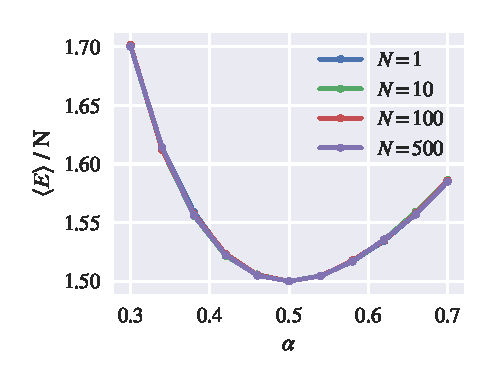
\includegraphics{figures/part_b/E_vs_alphas.eps}
        \caption{Mean energy, per particle, computed by VMC, for the non-interacting case, versus the variational parameter, \(\alpha\), for different number of particles \(N\). This is for a 3-dimensional system. We used \(2^{23}\) MC cycles for these computations.}
        \label{fig:mean_E_vs_alpha}
    \end{figure}
    
    Another result from the variational principle, states that the exact energy ground state will have a standard deviation of 0, an that this, as well as the energy, is a convex function of \(\alpha\). Table \ref{tab:validation_table}, compares the energy and standard deviations from the variational principle \(\sigma\) and from the blocking method \(\sigma_b\) for different values of \(\alpha\). We can see that the standard deviation is zero for \(\alpha = 0.5\). 
    
    \begingroup
    \setlength{\tabcolsep}{8pt} % Default value: 6pt
    \renewcommand{\arraystretch}{1.25} % Default value: 1
    \begin{table}
        \caption{Comparison of the mean energy, standard deviation, standard deviation by blocking and computational time in seconds, for different values of the variational parameter \(\alpha\). This is for a 3-dimensional non-interacting system with 100 particles. We used \(2^{23}\) MC cycles for these computations.}
        \begin{tabular}{c||cccc}
            \(\alpha\) & \(\langle E \rangle\) & \(\sigma\) & \(\sigma_b\) & t (s) \\ \hline \hline
            0.3 & 170.153772 & 6.553842 & 0.003200 & 8.925 \\ 
            0.34 & 161.206845 & 4.841202 & 0.002364 & 8.854 \\
            0.38 & 155.716986 & 3.390264 & 0.001655 & 8.862 \\ 
            0.42 & 152.323056 & 2.076341 & 0.001014 & 8.855 \\ 
            0.46 & 150.546719 & 1.034160 & 0.000505 & 8.853 \\ 
            0.5 & 150.000000 & 0.000000 & 0.000000 & 8.860 \\ 
            0.54 & 150.443678 & 0.938384 & 0.000458 & 8.859 \\ 
            0.58 & 151.764791 & 1.811414 & 0.000884 & 8.856 \\ 
            0.62 & 153.496155 & 2.716655 & 0.001326 & 8.858 \\ 
            0.66 & 155.777966 & 3.451178 & 0.001685 & 8.857 \\ 
            0.7 & 158.578630 & 4.141993 & 0.002022 & 8.858 \\ 
        \end{tabular}
        \label{tab:validation_table}
    \end{table}
    \endgroup
    
    In Figure \ref{fig:mean_E_vs_mc_cycles}, we can see equilibration process of the Markov chain as the number of cycles increases. As the simulation progresses, the Markov chain will reach the equilibrium state, i.e., where the energy will have less fluctuations. 
    
    \begin{figure}
        \centering
        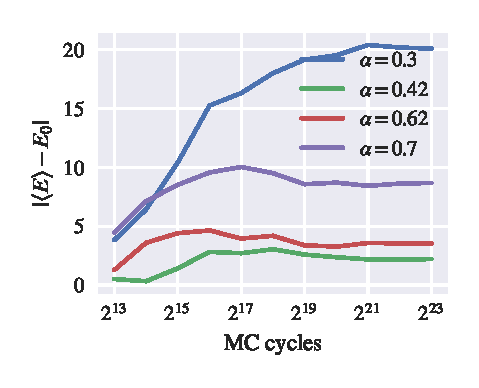
\includegraphics{figures/part_b/E_vs_mc_cycles.eps}
        \caption{Absolute different in the mean energy computed by VMC \(\langle E \rangle\) and the exact energy \(E_0\), for the non-interacting case, versus the number of MC cycles, for different values of the variational parameter \(\alpha\). This is for a 3-dimensional system with \(N=100\) particles. We used stated computing sampling the energy after \(2^{10}\) MC cycles.}
        \label{fig:mean_E_vs_mc_cycles}
    \end{figure}
    
    With these results, we have showed that our implementation produces the expected results for the mean energy as a function of the variational parameter, and that it can compute correctly the ground state energy for the optimal value of the variational parameters. Furthermore, we have seen the equilibration process of our Markov chain.
    
\section*{Sampling Routines}

    Having validated our implementation, we now compare both sampling routines, the Metropolis and Metropolis with importance sampling.

    In the Metropolis sampling routine, we update the position of each particle at random in an interval between \([-\text{sl}, \text{sl}]\), where sl is the step length. If the value of the sl is too small, we would be hard-pressed to explore a large region of the position space in reasonable MC time. We would, however, see a higher acceptance ratio of the trial moves. With a higher sl value, the acceptance ratio would be lower, but, the phase space explored would be larger. In Table \ref{tab:metrop}, we can see the comparison of simulation results for different values of the sl parameter. For the lower values of sl, the energy seems to vary more, while at the larger values it stays constant. This is due to the low volume of the explored phase space. The acceptance ratio also decreases with the increase of sl, meaning that we would need more steps to reach the equilibrium state.

    \begingroup
    \setlength{\tabcolsep}{2pt} % Default value: 6pt
    \renewcommand{\arraystretch}{1.25} % Default value: 1
    \begin{table}[]
        \caption{Simulational data for the Metropolis sampling for different step length (sl) values. It is presented the mean energy, standard deviation, standard deviation by blocking, the acceptance ratio and the computational time in seconds. These are results for \(\alpha = 0.66\), and \(2^{23}\) MC cycles.}
        \begin{tabular}{c||ccccc}
            step length & \(\langle E \rangle\) & \(\sigma\) & \(\sigma_b\) & \(A\) & t (s) \\ \hline \hline
            0.05 & 154.936919 & 3.544980 & 0.001731 & 0.984 & 13.470 \\
            0.1 & 156.333407 & 3.272738 & 0.001598 & 0.969 & 13.342 \\
            0.5 & 155.826593 & 3.455086 & 0.001687 & 0.845 & 13.108 \\
            1.0 & 155.858989 & 3.427333 & 0.001674 & 0.698 & 13.587 
        \end{tabular}
        \label{tab:metrop}
    \end{table}
    \endgroup

    We now shift our attention to Metropolis sampling with importance sampling. Instead of performing a unbiased random walk though the position space, we now update our system according to the Langevin equation \eqref{eq:langevin} and use the Green's Function from the Fokker-Plank equation \eqref{eq:gfs} to weigh our probability. Thus we move in the position space more efficiently, needing less steps to achieve the equilibrium stage. Meaning overall that our acceptance ratio of trial configurations to be higher. With this method, we have a parameter to tune, the \(\Delta t\) that comes from using Euler's method. If \(\Delta t\) is larger than unity, the Euler's method does not converges, thus our computations will be wrong. For lower values, \(\Delta t \in [0.01, 0.001]\), we can expect a high acceptance ratio.
    
    In Table \ref{tab:import}, shows simulation results for the Metropolis with importance sampling. As \(\Delta t\) increases, the acceptance ratio vanishes, because we will not be moving accordingly to the Langevin equation. This is due to the bad approximation by Euler's method. With a low enough \(\Delta t\) value, this method gives impressive results with an acceptance ratio of about \(1\). From this we would expect that the method will achieve the equilibrium regime in fewer MC cycles than the plain Metropolis, Figure \ref{fig:E_vs_mc_cycles_comp}.
    
    \begingroup
    \setlength{\tabcolsep}{4pt} % Default value: 6pt
    \renewcommand{\arraystretch}{1.25} % Default value: 1
    \begin{table}[]
        \caption{Simulational data for the Metropolis sampling with importance sampling for different \(\Delta t\) values. It is presented the mean energy, standard deviation, standard deviation by blocking, the acceptance ratio and the computational time in seconds. These are results for \(\alpha = 0.66\), and \(2^{23}\) MC cycles.}
        \begin{tabular}{c||ccccc}
            \(\Delta t\) & \(\langle E \rangle\) & \(\sigma\) & \(\sigma_b\) & \(A\) & t (s) \\ \hline \hline
            0.001 & 156.168450 & 3.562245 & 0.001739 & 1.000 & 10.452 \\
            0.01 & 155.870152 & 3.438343 & 0.001679 & 0.999 & 10.495 \\
            0.1 & 155.758238 & 3.451052 & 0.001685 & 0.978 & 10.462 \\
            1.0 & 155.835909 & 3.431596 & 0.001676 & 0.421 & 10.158 \\
            10.0 & 124.692469 & 0.290819 & 0.000142 & 0.000 & 10.429
        \end{tabular}
        \label{tab:import}
    \end{table}
    \endgroup

    % \begin{figure}
    %     \centering
    %     \includegraphics{figures/part_c/E_vs_alphas_comp.eps}
    %     \caption{Mean energy computed by VMC, with Metropolis sampling (sl\(=0.5\)) and Metropolis sampling with importance sampling (\(\Delta t = 0.1\)), versus the variational parameter \(\alpha\).  These are computations with \(2^{23}\) MC cycles.}
    %     \label{fig:E_vs_alphas_comp}
    % \end{figure}
    
    \begin{figure}
        \centering
        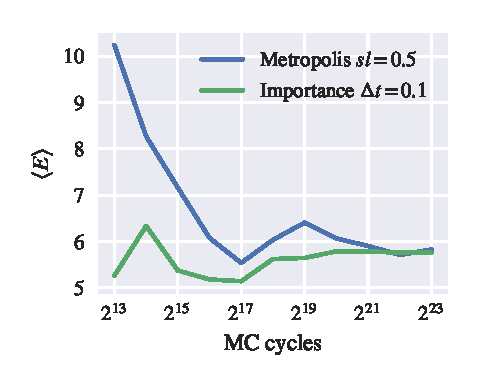
\includegraphics{figures/part_c/E_vs_mc_cycles_comp.eps}
        \caption{Mean energy as a function of the number of MC cycles, for the two different samplers, Metropolis (sl\(=0.5\)) and Metropolis with importance sampling (\(\Delta t = 0.1\)). Averages were taken since \(2^{12}\) MC cycles. These are results for \(\alpha = 0.66\).}
        \label{fig:E_vs_mc_cycles_comp}
    \end{figure}
    
    % \begin{figure}
    %     \centering
    %     \includegraphics{figures/part_c/std_E_vs_mc_cycles_comp.eps}
    %     \caption{Standard deviation of the energy as a function of the number of MC cycles, for the two different samplers, Metropolis (sl\(=0.5\)) and Metropolis with importance sampling (\(\Delta t = 0.1\)). Averages were taken since \(2^{12}\) MC cycles. These are results for \(\alpha = 0.66\).}
    %     \label{fig:std_E_vs_mc_cycles_comp}
    % \end{figure}

\section*{Interacting System}

    Having validated the implementation of VMC and analysed the differences between the two samplers, we study the interacting system of hard-core bosons. We now will consider an elliptical trap, of frequency \(\lambda = \sqrt{8}\), and the hard-core radius \(a = 0.00433\). For these calculations we used the Metropolis sampling with importance sampling, with \(\Delta t = 0.001\), for a high acceptance ratio and fast convergence.
    
    Now that we do not know the analytical solution to the problem, we can not determine analytically the optimal variational parameter. We used the gradient descent method, for a system with \(N=10\) in 3-dimensions, and found that
    \begin{equation*}
        \alpha_{opt} = 0.5054.
    \end{equation*}
    This is expected, since the elliptical trap shares a lot of similarities with the spherical one and that the interacting is very weak, \(a \sim 0\).
    
    \begingroup
    \setlength{\tabcolsep}{3pt} % Default value: 6pt
    \renewcommand{\arraystretch}{1.25} % Default value: 1
    \begin{table}[]
        \caption{Simulation results for the interacting hard-sphere bosons in a elliptical trap, for different particle counts. There results are for \(\alpha = 0.5054\) and with \(2^{20}\) MC cycles.}
        \begin{tabular}{c||ccccc}
        \(N\) & \(\langle E \rangle\) & \(\langle E \rangle / N\) & \(\sigma\) & \(\sigma_b\) & t (s) \\ \hline \hline
        10 & 24.316248 & 2.431625 & 0.103839 & 0.000143 & 4.134 \\
        50 & 125.106603 & 2.502132 & 0.330814 & 0.000457 & 3231.873 \\
        100 & 258.204285 & 2.582043 & 0.733256 & 0.001013 & 15365.751
        \end{tabular}
        \label{tab:E_int}
    \end{table}
    \endgroup
    
    \begingroup
    \setlength{\tabcolsep}{6pt} % Default value: 6pt
    \renewcommand{\arraystretch}{1.25} % Default value: 1
    \begin{table}[]
        \caption{Comparison of the mean energy between a system of interacting and non interacting bosons trapped in an elliptical harmonic oscillator. The \(\alpha\) value used was \(0.5054\).}
        \begin{tabular}{ccccc}
                                   & \multicolumn{2}{c}{Interacting}      & \multicolumn{2}{c}{Non Interacting}  \\ \hline \hline
        \multicolumn{1}{c||}{\(N\)} & \(\langle E \rangle\) & \(\sigma_b\) & \(\langle E \rangle\) & \(\sigma_b\) \\ \hline \hline
        \multicolumn{1}{c||}{10}  &    24.316248     &  0.000143   &      24.147619      &   0.000494   \\
        \multicolumn{1}{c||}{50}  &   125.106603         &   0.000457   &    120.708639       &    0.001078 \\
        \multicolumn{1}{c||}{100} &    258.204285        &  0.001013   &                       &             
        \end{tabular}
        \label{tab:comp_E_int}
    \end{table}
    \endgroup
    
    Results for simulations with the found optimal variational parameter \(\alpha_{opt}\), for different system sizes, \(N = \{10, 50, 100\}\), are shown in Table \ref{tab:E_int}. The mean energy per particle \(\langle E \rangle / N\), in this case, is not constant, since the energy, now, is dependent on the number of interactions. This effect would be better observed for larger systems, as shown in ref \cite{bec-trapped-bosons}. On Table \ref{tab:comp_E_int}, we can see the comparison between the energies of a interacting and non interacting system. 
    
    In Figure \ref{fig:one_body_densities}, we can see the one body densities for the system with and without interaction. The for a theoretical calculation, we would expect that the one body density for the interacting case to be spaced our over more positions. This happens because the particles can not the on top of one another, so they, naturally, space out. Here it is hard to see that effect, since we have to approximate the integral in Equation \eqref{eq:one_body} by the Monte-Carlo method.
    
    \begin{figure}
        \centering
        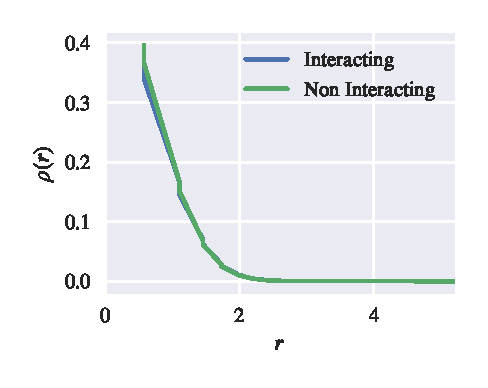
\includegraphics{figures/part_g/one_body_densities.eps}
        \caption{One body densities for the interacting and non interacting case, for a system with 10 particles.}
        \label{fig:one_body_densities}
    \end{figure}
    
    \section*{Conclusion}
    
    In this work we developed a Variational Monte Carlo code, for a system of interacting hard-core bosons trapped in an harmonic potential. We validated our implementation and discussed two different ways of sampling the positions space. We added the interaction term and computed the ground state energy for different system sizes and found that the energy per particle increases as we increase the number of particles. Since the interaction is weak, the differences in energy between the interactive and non interactive case are very small.

    \bibliography{refs}
    
\end{document}
